\chapter{Marco Metodológico}


\section{Metodología Tradicional} 
\subsection{RUP}

 RUP es un proceso para el desarrollo de un proyecto de software que define claramente quien, cómo, cuándo y qué debe hacerse en el proyecto, con 3 características esenciales, está dirigido por:

\begin{itemize}

    \item Los Casos de Uso : que orientan el proyecto a la importancia para el usuario y lo que este quiere. 

    \item La arquitectura: que Relaciona la toma de decisiones que indican cómo tiene que ser construido el sistema y en qué orden.

    \item Iterativo e incremental: dividiéndose el proyecto en mini proyectos donde los casos de uso y la arquitectura cumplen sus objetivos de manera más depurada.

\end{itemize}


\subsubsection{Ciclo de vida}
RUP divide el proceso en 4 fases, dentro de las cuales se realizan varias iteraciones en número variable según el proyecto y en las que se hace un mayor o menor hincapié en los distintas actividades
% \begin{figure}[!htb]
% 	\minipage{0.15\textwidth}
% 	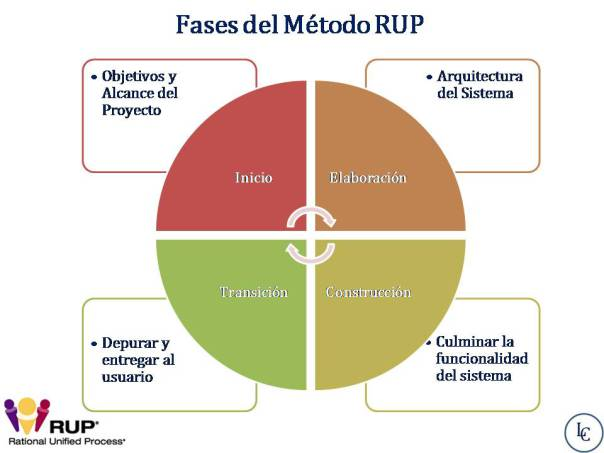
\includegraphics[width=\linewidth]{img/fases-rup.jpg}
% 	\endminipage\hfill
	
% \end{figure}

\begin{center}
	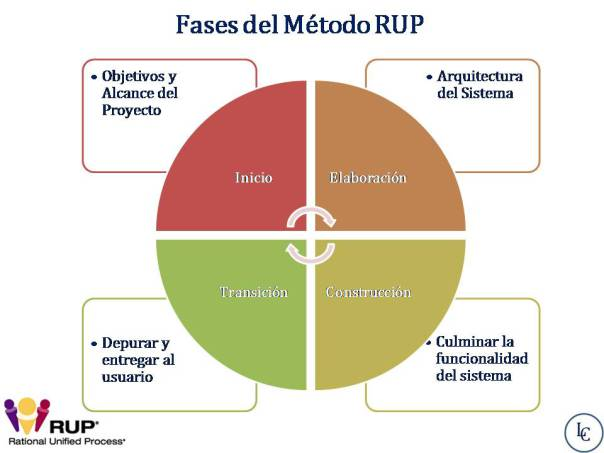
\includegraphics[width=13cm,height=8cm]{img/fases-rup.jpg}
\end{center}


\begin{itemize}

    \item Fase de Inicio: Esta fase tiene como propósito definir y acordar el alcance del proyecto con los patrocinadores, identificar los riesgos asociados al proyecto, proponer una visión muy general de la arquitectura de software y producir el plan de las fases y el de iteraciones posteriores.

	\item Fase de elaboración: En la fase de elaboración se seleccionan los casos de uso que permiten definir la arquitectura base del sistema y se desarrollaran en esta fase, se realiza la especificación de los casos de uso seleccionados y el primer análisis del dominio del problema, se diseña la solución preliminar.

	\item Fase de Desarrollo: El propósito de esta fase es completar la funcionalidad del sistema, para ello se deben clarificar los requisitos pendientes, administrar los cambios de acuerdo a las evaluaciones realizados por los usuarios y se realizan las mejoras para el proyecto.

	\item Fase de Transición: El propósito de esta fase es asegurar que el software esté disponible para los usuarios finales, ajustar los errores y defectos encontrados en las pruebas de aceptación, capacitar a los usuarios y proveer el soporte técnico necesario. Se debe verificar que el producto cumpla con las especificaciones entregadas por las personas involucradas en el proyecto.	

\end{itemize}
\subsection{Cuadro Comparativo}




\section{Metodología Ágil} 

El desarrollo ágil de software envuelve un enfoque para la toma de decisiones en los proyectos basados en el desarrollo iterativo e incremental, donde los requisitos y soluciones evolucionan con el tiempo según la necesidad del proyecto. Así el trabajo es realizado mediante la colaboración de equipos auto-organizados y multidisciplinarios, inmersos en un proceso compartido de toma de decisiones a corto plazo.

\subsection{SCRUM}
\subsubsection{Ciclo de vida}

\begin{center}
	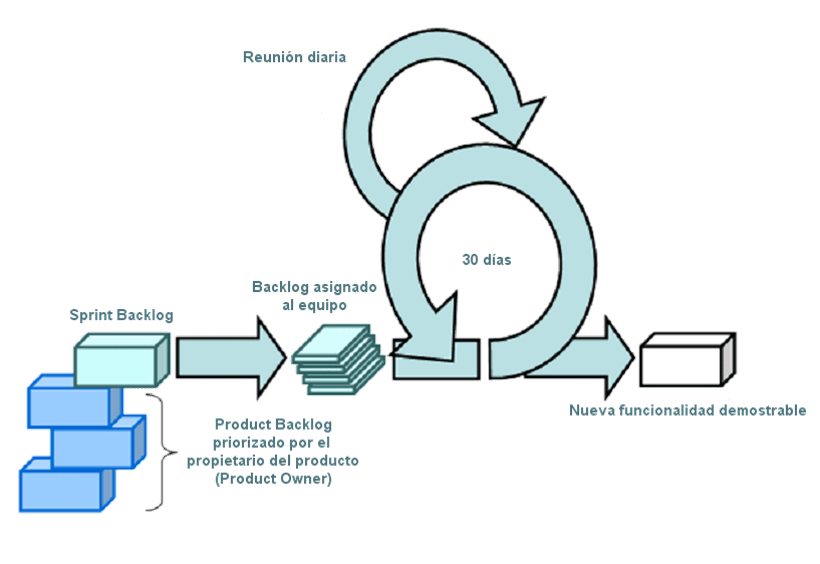
\includegraphics[width=13cm,height=8cm]{img/scrum.png}
\end{center}

\subsubsection{Spring}
\setlength{\parskip}{5mm}

	Es el periodo de tiempo durante el que se desarrolla un incremento de funcionalidad dura máximo 30 días. Constituye el núcleo de Scrum, que divide de esta forma el desarrollo de un proyecto en un conjunto de pequeñas “carreras”. Durante el proceso no se puede modificar el trabajo que se ha acordado en el Backlog, solo es posible cambiar el curso de un sprint abortándolo y esto solo puede hacerlo el Scrum Master. 
	
\setlength{\parskip}{0mm}

\subsubsection{}
    

\subsection{XP}

Es una metodología ágil centrada en potenciar las relaciones interpersonales como clave para el éxito en desarrollo de software, promoviendo el trabajo en equipo, preocupándose por el aprendizaje de los desarrolladores, y propiciando un buen clima de trabajo. XP se basa en realimentación continua entre el cliente y el equipo de desarrollo, comunicación fluida entre todos los participantes, simplicidad en las soluciones implementadas y coraje para enfrentar los cambios. XP se define como especialmente adecuada para proyectos con requisitos imprecisos, muy cambiantes, y donde existe un alto riesgo técnico.

\subsubsection{Prácticas básicas de la programación extrema}


\begin{itemize}

    \item Equipo completo: Forman parte del equipo todas las personas que tienen algo que ver con el proyecto, incluido el cliente y el responsable del proyecto. 

	\item Planificación: Se hacen las historias de usuario y se planifica en qué orden se van a hacer y las mini-versiones. La planificación se revisa continuamente. 
	
	\item Test del cliente: El cliente, con la ayuda de los desarrolladores, propone sus propias pruebas para validar las mini-versiones. 

	\item Versiones pequeñas: Las mini-versiones deben ser lo suficientemente pequeñas como para poder hacer una cada pocas semanas. Deben ser versiones que ofrezcan algo útil al usuario final y no trozos de código que no pueda ver funcionando. 

	\item Diseño simple: Hacer siempre lo mínimo imprescindible de la forma más sencilla posible. Mantener siempre sencillo el código. 

	\item Pareja de programadores: Los programadores trabajan por parejas (dos delante del mismo ordenador) y se intercambian las parejas con frecuencia (un cambio diario). 

	\item Desarrollo guiado por las pruebas automáticas: Se deben realizar programas de prueba automática y deben ejecutarse con mucha frecuencia. Cuantas más pruebas se hagan, mejor. 

	\item Integración continua: Deben tenerse siempre un ejecutable del proyecto que funcione y en cuanto se tenga una nueva pequeña funcionalidad, debe recompilarse y probarse. Es un error mantener una versión congelada dos meses mientras se hacen mejoras y luego integrarlas todas de golpe. Cuando falle algo, no se sabe qué es lo que falla de todo lo que hemos metido. 

	\item El código es de todos: Cualquiera puede y debe tocar y conocer cualquier parte del código. Para eso se hacen las pruebas automáticas. 

	\item Normas de codificación: Debe haber un estilo común de codificación (no importa cual), de forma que parezca que ha sido realizado por una única persona. 

	\item Metáforas: Hay que buscar unas frases o nombres que definan cómo funcionan las distintas partes del programa, de forma que sólo con los nombres se pueda uno hacer una idea de qué es lo que hace cada parte del programa. Un ejemplo claro es el "recolector de basura" de java. Ayuda a que todos los programadores (y el cliente) sepan de qué estamos hablando y que no haya mal entendidos. 

	\item Ritmo sostenible: Se debe trabajar a un ritmo que se pueda mantener indefinidamente. Esto quiere decir que no debe haber días muertos en que no se sabe qué hacer y que no se deben hacer un exceso de horas otros días. Al tener claro semana a semana lo que debe hacerse, hay que trabajar duro en ello para conseguir el objetivo cercano de terminar una historia de usuario o mini-versión. 


\end{itemize}



\subsubsection{Ciclo de vida}

\subsection{Agilus}
\subsection{Cuadro Comparativo}

\section{Cuadro comparativo [Metodologías Tradicionales vs Ágiles]} 


\begin{center}
\begin{tabular}{ | m{6cm} | m{6cm} | } 
 \hline
 Tradicionales & Ágiles \\ 
	\hline
	Basadas en normas provenientes de estándares seguidos por el entorno de desarrollo.  Posee cierta resistencia a los cambios. 
	&
	Basadas en heurísticas provenientes de prácticas de producción de código las cuales previenen cambios durante el proyecto.\\ 
 	\hline
 	Define un proceso mucho más controlado junto con numerosas políticas/normas.
	&
	Define un proceso menos controlado, con pocos principios.\\ 
	\hline
	El cliente interactúa con el equipo de desarrollo mediante reuniones.	
	&
	El cliente es parte del equipo de desarrollo. \\ 
	\hline
	Genera más artefactos.	
	&
	Genera pocos artefactos.\\ 
	\hline

	Más roles.	
	&
	Pocos roles.\\ 
	\hline

	Grupos grandes y posiblemente distribuidos.	
	&
	Grupos pequeños (<10 integrantes) y trabajando en el mismo sitio.\\ 
	\hline

	Dependencia de la arquitectura de software mediante modelos.	
	& 
	Menor dependencia de la arquitectura de software.\\ 
	\hline

	Existe un contrato prefijado.	
	&
	No existe contrato tradicional o al menos es bastante flexible.\\ 
	\hline

\end{tabular}
%\caption{Table to test captions and labels}
%\label{table:1}
\end{center}





